\section{Evaluation}

The survey where children, parents, and teachers participated was held online using Google Forms.
An equivalent face-to-face survey was also done with children.
Both groups showed, on average, the same results.

The assumptions before doing the survey were that at least 90 percent of respondents play non-educational games;
respondents (especially children) play some building games (such as Minecraft), children are mostly (at least 75 percent) competitive, and the most crucial aspect is the game itself, explanation, and a story.

The survey results pointed out that almost 22 percent of respondents do not play non-educational games.
Almost 18 percent of respondents (primarily children) play building games.
Respondents also chose to play casual games and shooting games in almost 14 percent of responses, puzzle or strategy games in nearly 12 percent of responses, board games, battle-royal-like games, and shooting games in about 7 percent.
The results of which non-educational games people play are shown in figure \ref{fig:survey:games}.

\begin{figure}
    \centering
    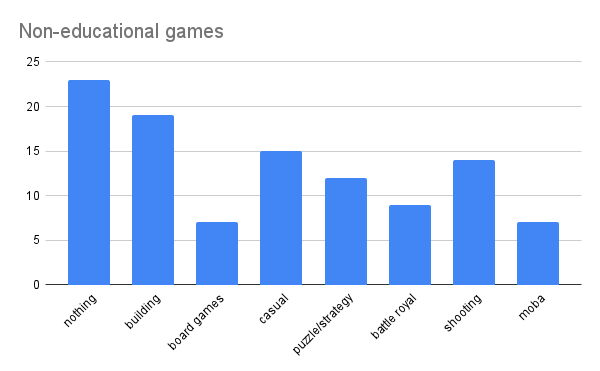
\includegraphics[width=1\linewidth]{assets/survey/non-educational-games.png}
    \caption{Played Non-educational Types of Games}
    \label{fig:survey:games}
\end{figure}

In a matter of educational games people use, almost 60 percent of respondents use Duolingo~-- language learning educational game.
Almost 30 percent of respondents also selected Minecraft~-- a game known for its building mechanics and an option to program with unique blocks.
Almost 15 percent of respondents use Scratch~-- a tool to do visual programming.
Other minor answers were, for example, Khan Academy and Kahoot with almost 7 percent.  

Focusing on children's answers, almost 80 percent like receiving some reward for completing tasks; nearly 75 percent like rating systems; and almost 80 percent of respondents would like the last task to be a challenge.

Questions about what aspects or mechanics are important in an educational game showed exciting differences.
While children selected with the same share a game, a story, and an explanation, almost none selected study materials.
Parents and teachers selected a story and an explanation, while almost none chose a game and study materials.
Interestingly, the difference between children and parents or teachers is the view on the importance of the game aspects.

The results and initial assumptions contradict that most people play non-educational games; confirm that building games are the most common kind of games children play; and show that children are -- majority with almost 75 percent -- competitive. 

The conducted survey with the addition of articles mentioned in the introduction suggests that gamification in educational games might introduce valuable benefits.
In summary, children like to receive rewards in some form of points, want to compete and be rated, and like challenges.
All these factors underline the motivational aspects found in mentioned studies,
as they help to increase the attention span.
